\subsection{(a) & (b) & (c)}

I estimate the equation in problem 1 (a) by including only second lags (specification 1) and by including second and third lags (specification 2). Specification 3 is autocorrelated transmitted shocks without fixed effects (the selected $\rho=0.758$) and specification 4 (the selected $\rho=1.159$) is autocorrelated transmitted shocks with fixed effects.


\begin{figure}[h!]
    \centering
    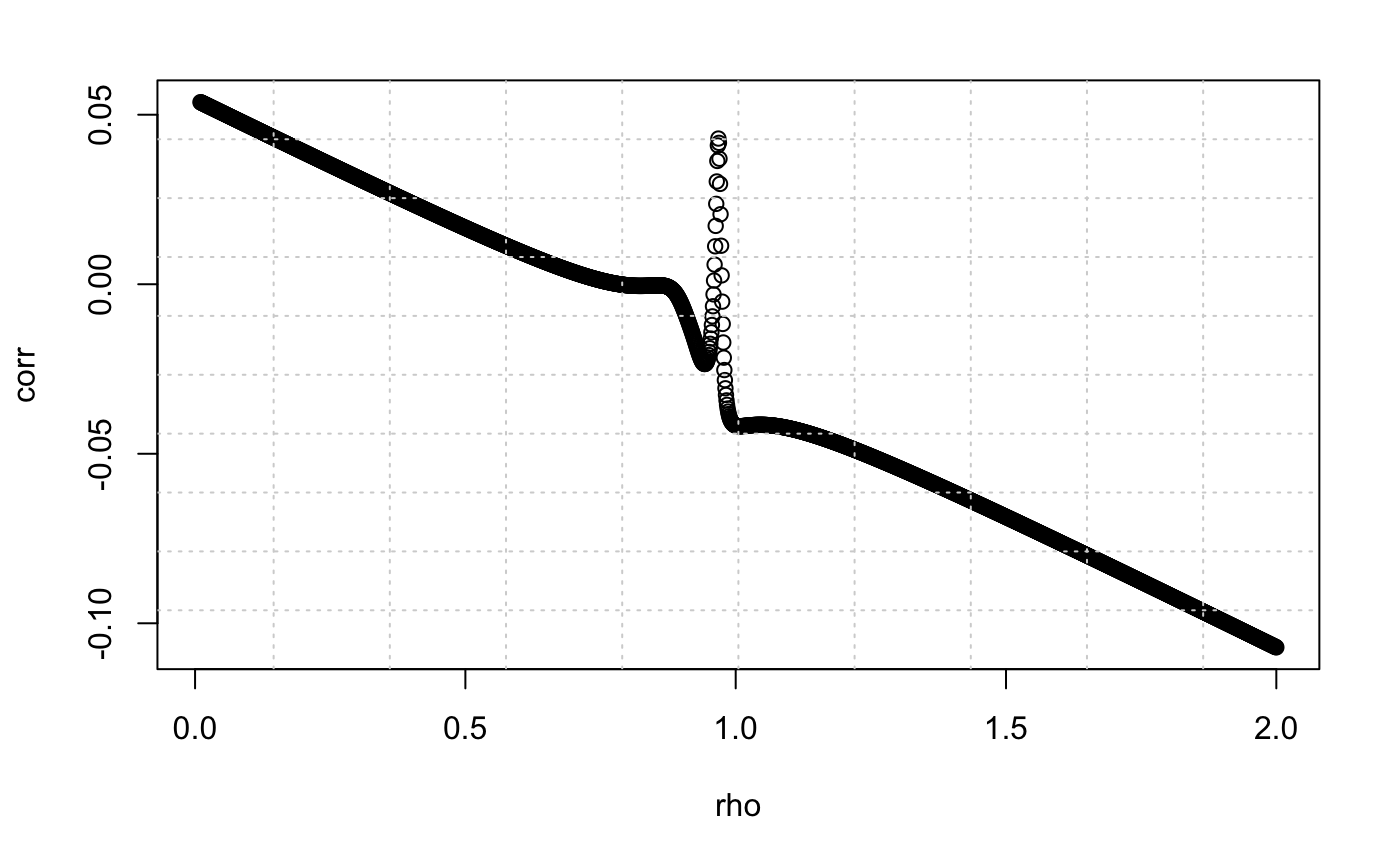
\includegraphics[scale=0.15]{HW2/Attachments/Q1b.png}
    \caption{Moment Condition vs $\rho$ for (b)}
    \label{fig:my_label}
\end{figure}

\begin{figure}[h!]
    \centering
    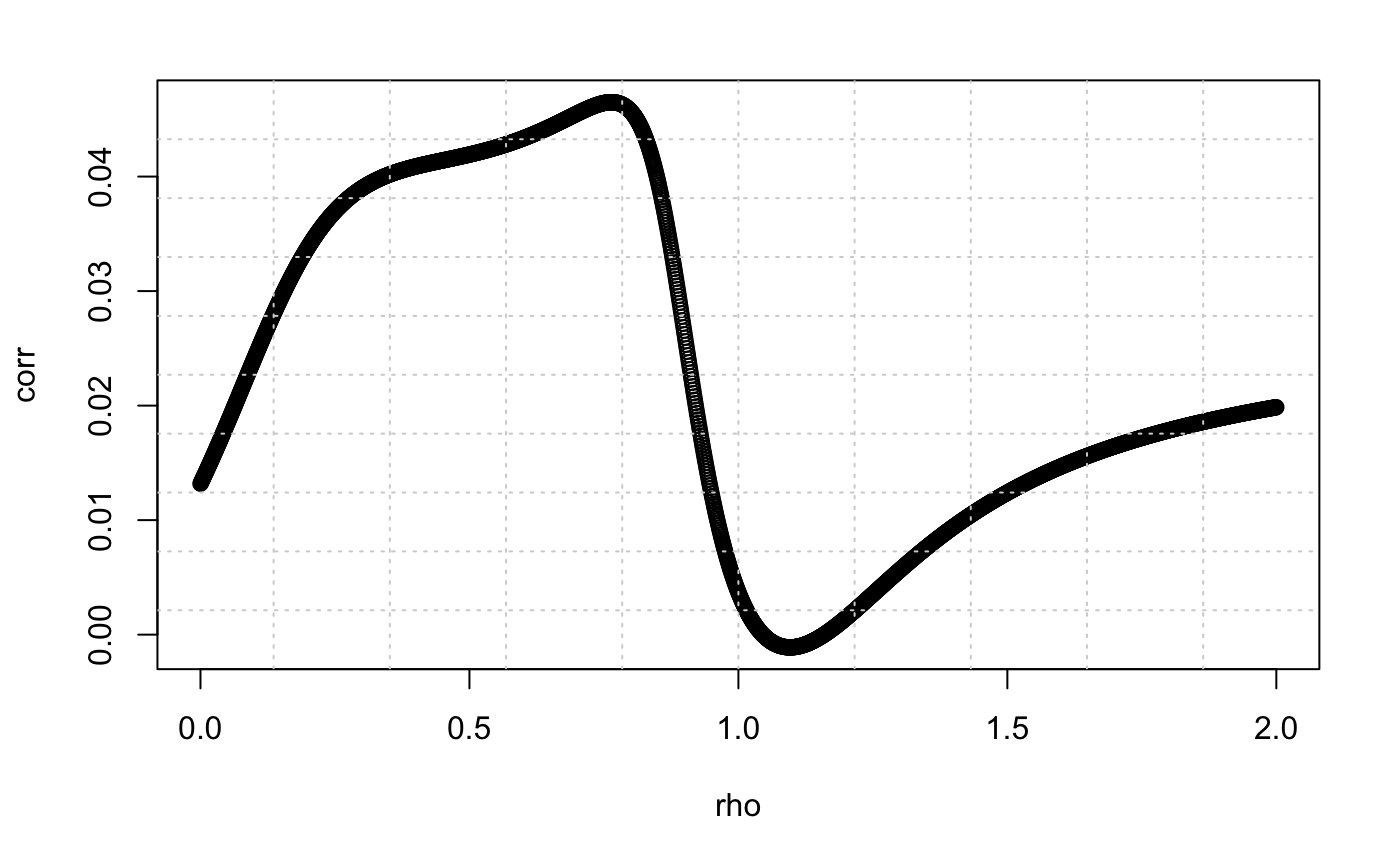
\includegraphics[scale=0.15]{HW2/Attachments/Q1c.png}
    \caption{Moment Condition vs $\rho$ for (c)}
    \label{fig:my_label}
\end{figure}

\begin{table}[h!]
    \centering
    \footnotesize{
    {
\def\sym#1{\ifmmode^{#1}\else\(^{#1}\)\fi}
\begin{tabular}{l*{4}{c}}
\hline\hline
            &\multicolumn{1}{c}{(1)}&\multicolumn{1}{c}{(2)}&\multicolumn{1}{c}{(3)}&\multicolumn{1}{c}{(4)}\\
            &\multicolumn{1}{c}{IV Regressions with 2L}&\multicolumn{1}{c}{IV Regressions with 3L}&\multicolumn{1}{c}{AR Shocks}&\multicolumn{1}{c}{AR Shocks+FE}\\
\hline
lemp        &       0.221         &       0.661         &       0.517\sym{***}&      -1.076         \\
            &      (0.68)         &      (1.85)         &      (3.65)         &     (-0.25)         \\
[1em]
ldnpt       &       0.869\sym{**} &      -0.269         &       0.439\sym{***}&       4.013         \\
            &      (2.78)         &     (-0.68)         &      (4.54)         &      (0.56)         \\
[1em]
ldrst       &      -0.555         &       0.409         &      0.0963         &       0.221         \\
            &     (-1.70)         &      (1.34)         &      (1.32)         &      (0.03)         \\
[1em]
d73         &           0         &           0         &           0         &           0         \\
            &         (.)         &         (.)         &         (.)         &         (.)         \\
[1em]
d78         &           0         &           0         &           0         &           0         \\
            &         (.)         &         (.)         &         (.)         &         (.)         \\
[1em]
d83         &      -0.633\sym{***}&           0         &      -0.390\sym{***}&           0         \\
            &     (-4.46)         &         (.)         &    (-11.21)         &         (.)         \\
[1em]
d88         &           0         &           0         &           0         &           0         \\
            &         (.)         &         (.)         &         (.)         &         (.)         \\
[1em]
d357\_73     &           0         &           0         &           0         &           0         \\
            &         (.)         &         (.)         &         (.)         &         (.)         \\
[1em]
d357\_78     &           0         &           0         &           0         &           0         \\
            &         (.)         &         (.)         &         (.)         &         (.)         \\
[1em]
d357\_83     &       1.471\sym{***}&           0         &       0.853\sym{***}&           0         \\
            &     (13.80)         &         (.)         &     (16.92)         &         (.)         \\
[1em]
d357\_88     &       1.087\sym{***}&       0.903\sym{***}&       0.810\sym{***}&      -0.798         \\
            &     (10.69)         &      (8.71)         &     (15.09)         &     (-0.75)         \\
[1em]
\_cons      &       0.474\sym{***}&       0.161         &       0.820\sym{***}&       1.959         \\
            &      (4.66)         &      (1.66)         &     (10.55)         &      (0.68)         \\
\hline
\(N\)       &         682         &         214         &         682         &         214         \\
\hline\hline
\multicolumn{5}{l}{\footnotesize \textit{t} statistics in parentheses}\\
\multicolumn{5}{l}{\footnotesize \sym{*} \(p<0.05\), \sym{**} \(p<0.01\), \sym{***} \(p<0.001\)}\\
\end{tabular}
}

    }
    \caption{Question 1}
    \label{tab:my_label}
\end{table}

\subsection{(d)}

As we can see from Table 1, specifications (1) and (2) do not make much sense: in specification (1), the coefficient on R\&D capital is negative, while in specification (2) the coefficient on capital is negative. The first stage of both these regressions suggests that the instruments might be weak: the F-statistic of the first stage is around 10 in specification (1) and much lower than 10 in specification (2).

The results of specification (3) seem much more reasonable compared to specifications (1) and (2), suggesting that the assumption of no autocorrelation in the transmitted shock is restrictive. The estimated autocorrelation is $\rho=0.758$, which is a high coefficient, so ignoring it results in a seriously biased estimates.

The results of specification (4) are also not reasonable: they suggest that nothing is significant. Including fixed effects forces us to (i) use only a balanced panel for estimation, reducing the sample size threefold, and (ii) use higher-order lags for estimation which makes them weaker instruments. That is, on this sample, accounting for fixed effects creates more problems than it solves.
